\documentclass[lettersize,journal]{IEEEtran}

% -------- Packages (matching Paper 1) --------
\usepackage{amsmath,amsfonts}
\usepackage{array}
\usepackage[caption=false,font=normalsize,labelfont=sf,textfont=sf]{subfig}
\usepackage{textcomp}
\usepackage{stfloats}
\usepackage{url}
\usepackage{verbatim}
\usepackage{graphicx}
\usepackage{cite}
\usepackage{afterpage}
\usepackage[T1]{fontenc}
\usepackage{longtable}
\usepackage{booktabs}
\usepackage[english]{babel}
\addto\captionsenglish{\renewcommand{\figurename}{Fig.}}
\usepackage{xcolor}
\usepackage{tikz}
\usetikzlibrary{arrows.meta,positioning}
\usepackage[hidelinks]{hyperref}
\usepackage{makecell}
\usepackage{mathtools}

% -------- Draft helpers --------
% Placeholder for results to be inserted after the modelling is complete.
\newcommand{\tbd}[1]{\textcolor{red}{[#1]}}

% -------- Settings --------
\setlength{\jot}{2pt}
\allowdisplaybreaks[1]
\hyphenation{op-tical net-works semi-conduc-tor IEEE-Xplore}
% Allow long bibliography URLs to break at hyphens and slashes
\Urlmuskip=0mu plus 1mu\relax
\def\UrlBreaks{\do\/\do\-\do\_\do\.\do\=\do\&}

\begin{document}

% -------- Title/Author --------
\title{Revenue Stacking of Data Centre Flexibility in the Reformed Great Britain Electricity Markets}

\author{James Day\textsuperscript{1}, Mehmet Turker Takci\textsuperscript{1}, and Meysam Qadrdan\textsuperscript{1}}

\IEEEaftertitletext{%
  \vspace{-0.5em}%
  \noindent\small
  \textsuperscript{1}Cardiff University, Queen's Buildings, The Parade, Cardiff CF24 3AA, United Kingdom\par
  \vspace{0.6em}
  \noindent\small\textbf{Corresponding author:}\par
  \vspace{0.1em}
  \noindent\small
  James Day\par
  \textit{E-mail address:} \texttt{DayJa1@cardiff.ac.uk}\par
  \vspace{0.6em}
}

\maketitle

\markboth{Journal of \LaTeX\ Class Files,~Vol.~XX, No.~XX, 2026}%
{Day \MakeLowercase{\textit{et al.}}: Revenue Stacking of Data Centre Flexibility in the Reformed GB Electricity Markets}

% -------- Abstract & Keywords --------
\begin{abstract}
Data centres are the fastest growing category of electricity demand in Great Britain, with approximately 50~GW of proposed capacity in the connection queue, yet the system operator's Future Energy Scenarios currently assume that none of their demand-side flexibility materialises, citing a lack of evidence. Over the same period, the GB balancing services landscape has been comprehensively rebuilt: frequency response is now procured through co-optimised day-ahead auctions, an entirely new reserve family has been introduced, the Demand Flexibility Service has become a year-round, bi-directional product, and independent aggregators have gained access to the wholesale market. Meanwhile, the abolition of Triad avoidance has invalidated the revenue assumptions underpinning much of the existing data centre flexibility literature. This paper presents, to the authors' knowledge, the first revenue-stacking framework that co-optimises a whole-facility data centre model, comprising deferrable IT workload, uninterruptible power supply (UPS) battery storage and a cooling system with thermal energy storage, across the full post-reform GB product set: day-ahead energy arbitrage, dynamic frequency response, the new reserve services, the Balancing Mechanism, the Demand Flexibility Service, the Capacity Market and distribution-level flexibility. Capacity commitments are coupled to the facility's physical schedule through shared headroom, per-asset allocation and stored-energy reservation constraints, and every committed megawatt is certified as deliverable for its product's required duration from any callable state using the magnitude--duration flexibility envelope developed in our companion work. Because the GB products clear at different market gates, the co-optimised portfolio is interpreted as a full-information upper bound and benchmarked against a market-sequential implementation in which the day-ahead energy position and availability commitments are fixed before Balancing Mechanism and Demand Flexibility Service decisions are taken over the residual certified headroom. Uncertainty in prices and service utilisation is captured through a two-stage stochastic extension with conditional value-at-risk. The framework is applied to a 10~MW data centre using 2024--2026 GB market data. Results show that the value-maximal portfolio yields \tbd{XX~\pounds k/MW/yr}, a \tbd{XX\%} uplift on energy-only optimisation, that uncertified stacking would oversell deliverable flexibility by \tbd{XX\%}, and that the optimal stack is layered by response speed, with the UPS backing dynamic response, IT workload shifting backing energy, reserve and capacity products, and thermal storage extending deliverable durations. The framework provides the quantified, duration-certified evidence base that system operators and policymakers require to integrate flexible data centres into markets and connection arrangements.
\end{abstract}

\begin{IEEEkeywords}
Data centre, Demand-side flexibility, Revenue stacking, Ancillary services, Electricity markets, Great Britain
\end{IEEEkeywords}

% -------- Nomenclature --------
\afterpage{
\clearpage
\onecolumn
{\small
\renewcommand{\arraystretch}{1.15}
\begin{longtable}{p{0.13\textwidth} p{0.63\textwidth} p{0.12\textwidth} p{0.06\textwidth}}
\caption{Nomenclature (facility-model symbols follow the companion paper \cite{takci2026characterisation}; only symbols used in this paper are listed)} \label{tb:nomenclature} \\
\toprule
\textbf{Symbol} & \textbf{Definition} & \textbf{Value/Bounds} & \textbf{Unit} \\
\midrule
\endfirsthead
\multicolumn{4}{c}%
{{\bfseries \tablename\ \thetable{} -- continued from previous page}} \\
\toprule
\textbf{Symbol} & \textbf{Definition} & \textbf{Value/Bounds} & \textbf{Unit} \\
\midrule
\endhead
\midrule
\multicolumn{4}{r}{{Continued on next page}} \\
\endfoot
\bottomrule
\endlastfoot
\midrule
\multicolumn{4}{l}{\textbf{Sets and indices}} \\
\midrule
$t, s$ & Time slot indices over the extended planning horizon. & $\{1,\dots,108\}$ & -- \\
$T, T^{\mathrm{ext}}$ & 24-hour planning horizon and its 3-hour extension. & -- & -- \\
$\Delta t$ & Duration of a single time slot. & 0.25 & hours \\
$k \in K$ & Deferral tranche of a flexible IT job. & $\{1,\dots,4\}$ & -- \\
$j \in J$ & Market product index; $J = J^{\downarrow} \cup J^{\uparrow}$ for demand turn-down and turn-up products respectively. & -- & -- \\
$b \in B_j$ & Procurement window of product $j$ (EFA block for response, settlement period for Balancing Reserve, auction window otherwise); $b(t)$ denotes the window containing slot $t$. & -- & -- \\
$L_b$ & Length of procurement window $b$. & -- & hours \\
$a \in A$ & Facility asset: IT workload (IT), UPS battery (UPS), cooling with TES (CL). & -- & -- \\
$\mathcal{D}$ & Set of distinct product sustain durations, $\mathcal{D} = \{\tau_j : j \in J\}$. & -- & hours \\
$\omega \in \Omega$ & Scenario index (stochastic formulation); probability $p_\omega$. & -- & -- \\
\midrule
\multicolumn{4}{l}{\textbf{Market parameters}} \\
\midrule
$\tau_j$ & Required sustain duration of product $j$ at full committed output. & Table~\ref{tab:products} & hours \\
$\pi^{\mathrm{DA}}(t)$ & Day-ahead wholesale electricity price. & Varies & \pounds/MWh \\
$\pi^{\mathrm{N}}(t)$ & Time-varying residual network (DUoS) charge. & Varies & \pounds/MWh \\
$\pi^{\mathrm{av}}_{j,b}$ & Availability clearing price of product $j$ in window $b$. & Varies & \pounds/MW/h \\
$\pi^{\mathrm{ut}}_{j}$ & Utilisation price of product $j$. & Varies & \pounds/MWh \\
$\pi^{\mathrm{off}}(t), \pi^{\mathrm{bid}}(t)$ & Balancing Mechanism offer and bid prices. & Varies & \pounds/MWh \\
$\pi^{\mathrm{DFS}}, \pi^{\mathrm{DSO}}$ & Demand Flexibility Service and DSO service prices. & Varies & \pounds/MWh \\
$\pi^{\mathrm{CM}}$ & Capacity Market clearing price. & Varies & \pounds/kW/yr \\
$\varphi_j$ & Expected utilisation factor of product $j$ (fraction of committed capacity-hours called). & $[0,1]$ & -- \\
$\kappa$ & Balancing Mechanism acceptance factor. & $[0,1]$ & -- \\
$\delta^{\mathrm{CM}}$ & Capacity Market de-rating factor for demand-side response. & $[0,1]$ & -- \\
$P^{\mathrm{conn}}$ & Firm import capacity of the grid connection. & 12{,}000 & kW \\
$\mathbb{1}_{\mathrm{SS}}(t)$ & Indicator equal to 1 during Capacity Market stress-event and test windows. & $\{0,1\}$ & -- \\
\midrule
\multicolumn{4}{l}{\textbf{Decision variables (market layer)}} \\
\midrule
$r_{j,b}$ & Capacity committed to product $j$ in procurement window $b$. & $\geq 0$ & kW \\
$\beta^{a}_{j,b}$ & Share of commitment $r_{j,b}$ allocated to asset $a$. & $[0,1]$ & -- \\
$x^{\mathrm{off}}(t), x^{\mathrm{bid}}(t)$ & Balancing Mechanism offer (turn-down) and bid (turn-up) volumes delivered in slot $t$ (within-day recourse decisions). & $\geq 0$ & kW \\
$x^{\mathrm{dfs},\downarrow}(t), x^{\mathrm{dfs},\uparrow}(t)$ & DFS turn-down and turn-up delivery (event slots only; event-driven recourse decisions). & $\geq 0$ & kW \\
$x^{\mathrm{dso}}(t)$ & DSO flexibility delivery within tendered windows. & $\geq 0$ & kW \\
$C^{\mathrm{CM}}$ & Capacity Market committed capacity (annual outer decision). & $\geq 0$ & kW \\
\midrule
\multicolumn{4}{l}{\textbf{Derived quantities}} \\
\midrule
$P^{\mathrm{Grid}}(t)$ & Total facility power drawn from the grid. & $\geq 0$ & kW \\
$H^{a,\downarrow}(t), H^{a,\uparrow}(t)$ & Instantaneous turn-down and turn-up headroom of asset $a$. & $\geq 0$ & kW \\
$H^{\mathrm{IT},\downarrow}_{\tau}(t)$ & Duration-aware IT turn-down headroom sustainable for $\tau$ hours. & $\geq 0$ & kW \\
$u^{\mathrm{flr}}_{\tau}(t)$ & CPU-utilisation floor: utilisation that cannot be deferred by at least $\tau$ hours from slot $t$. & $[0,1]$ & -- \\
$P^{\mathrm{flr}}_{\tau}(t)$ & IT power corresponding to the utilisation floor $u^{\mathrm{flr}}_{\tau}(t)$. & $\geq 0$ & kW \\
$\overline{\Delta P}^{\downarrow}(t,\tau), \overline{\Delta P}^{\uparrow}(t,\tau)$ & Certified magnitude--duration envelope: maximum deviation sustainable for $\tau$ hours from slot $t$ \cite{takci2026characterisation}. & $\geq 0$ & kW \\
$C_\omega$ & Net daily operating cost in scenario $\omega$. & Varies & \pounds \\
$\zeta, \varsigma_\omega$ & CVaR auxiliary variables (value-at-risk level and scenario excess). & -- & \pounds \\
$\lambda$ & Risk-aversion weight. & $\geq 0$ & -- \\
$q$ & CVaR confidence level. & 0.95 & -- \\
\end{longtable}
\twocolumn
}
}

% ======================================================================
\section{Introduction}
% ======================================================================

\IEEEPARstart{D}{ata} centres are the fastest growing category of electricity demand in Great Britain. The National Energy System Operator (NESO) projects that GB data centre consumption will rise from 7.6~TWh in 2024 to around 33~TWh by 2035 \cite{neso2025fes}, and globally the IEA expects data centre demand to more than double by 2030, driven principally by artificial intelligence workloads \cite{iea_energy_ai}. The spatial concentration of this growth is placing acute pressure on network access: by mid-2025 the GB demand connection queue had tripled to approximately 125~GW, of which around 140 proposed data centre projects account for roughly 50~GW, exceeding the entire GB peak demand of about 45~GW \cite{neso2025connections,desnz2026strategicdemand}. Data centres are simultaneously one of the largest new burdens on the power system and, as our companion work demonstrates \cite{takci2026characterisation}, one of its most capable prospective providers of demand-side flexibility.

That capability, however, is currently valued at zero in the official planning evidence base. NESO's Future Energy Scenarios explicitly exclude data centre demand flexibility from all pathways, citing insufficient evidence that it will be offered \cite{neso2025fes,eca2025hole}. The consequence is a self-reinforcing omission: because flexibility is not credited, data centres are planned, connected and charged as inflexible loads, and because they are treated as inflexible, no revenue or connection benefit accrues to operators who could provide flexibility. Policy is now moving to break this circularity. Ofgem and the Department for Energy Security and Net Zero are developing arrangements under which large demand users who commit to flexible operation can receive accelerated network connections \cite{desnz2026strategicdemand,ofgem2025tm04}, and the Clean Flexibility Roadmap targets a doubling of GB flexible capacity by 2030 \cite{clean_flexibility_roadmap}. What is missing is a rigorous, market-specific quantification of what a flexible data centre is actually worth, and of how its internal assets should be deployed across the available products. Providing that quantification is the purpose of this paper.

The question of \emph{where} a data centre should sell its flexibility has become substantially more interesting, and more complicated, as a result of the comprehensive reform of the GB balancing and flexibility markets between 2023 and 2026. Frequency response is now procured through the Enduring Auction Capability (EAC), a co-optimised day-ahead auction across the three dynamic response services \cite{neso2026eac}. An entirely new reserve family has been introduced: Balancing Reserve (March 2024), Quick Reserve (phased in from late 2024) and Slow Reserve (replacing Short Term Operating Reserve) \cite{neso2026br,neso2026qr,neso2025srdesign}. The Demand Flexibility Service, originally a winter contingency product, has been redesigned as a year-round, bi-directional, zonally procured service open to assets as small as 0.1~MW \cite{neso2026dfsshakeup}. Independent aggregators have gained wholesale market access through modification P415 \cite{elexon2024p415}, and market-wide half-hourly settlement is universalising exposure to time-varying prices \cite{elexon2026mhhs}. In the opposite direction, the Targeted Charging Review abolished the Triad avoidance mechanism that dominated the business case in much of the earlier GB demand-side literature \cite{ofgem2019tcr}, and the 2025 decision to retain reformed national pricing rather than introduce zonal wholesale prices has settled the locational framework within which flexibility will be remunerated \cite{desnz2025rema}. Any credible valuation of data centre flexibility in GB must therefore be built on the post-reform product set; valuations calibrated to the pre-2023 market are obsolete in both directions, overstating network-charge revenues that no longer exist and omitting products that did not yet exist.

Monetising flexibility across many products simultaneously raises a problem that single-product studies do not face: the same physical capability must not be sold twice, and every committed megawatt must be genuinely deliverable. For a stand-alone battery, deliverability reduces to a simple comparison of energy capacity against power commitment, and a mature literature has developed revenue-stacking optimisations on this basis \cite{staffell2016maximising,seward2022revenue,pusceddu2021synergies,mohamed2023stacked}. A data centre is fundamentally harder. Its dominant flexible resource, deferrable IT workload, is not a battery: deferred computation must still be executed within contractual delay tolerances, so every reduction creates a rebound whose cost depends on future prices; its deliverable magnitude depends on how much deferrable work happens to be running; and its interaction with the cooling system means that the feasible envelope is shaped by thermal states and storage levels that evolve with the schedule itself. Our companion paper \cite{takci2026characterisation} showed that the feasible duration of a given power deviation varies by more than an order of magnitude with the time of day at which it is requested. A revenue-stacking model that ignores this structure will systematically sell flexibility that cannot be delivered, a failure mode we term \emph{phantom flexibility}, and one that recent work on data centre regulation bidding has begun to recognise in the single-service setting \cite{fan2026harnessing}.

This paper addresses these challenges by extending the whole-facility optimisation model and duration-aware flexibility assessment of \cite{takci2026characterisation} into a market-facing revenue-stacking framework. The facility's day-ahead energy position and its capacity commitments across the full post-reform GB product set are co-optimised subject to shared headroom constraints, per-asset allocation, and stored-energy reservations, and the resulting portfolio is certified against the magnitude--duration flexibility envelope so that every offer is deliverable for its product's required duration from any callable state. The main contributions are:
\begin{enumerate}
    \item a revenue-stacking formulation for a whole-facility data centre, co-optimising wholesale energy arbitrage with commitments to dynamic frequency response, the new GB reserve services, the Balancing Mechanism, the Demand Flexibility Service, the Capacity Market and distribution-level flexibility, together with a dated codification of the post-reform GB demand-side product set, its stacking rules and its clearing sequence, the last of which defines the model's decision stages;
    \item a duration-certification method that converts the magnitude--duration flexibility envelope of \cite{takci2026characterisation} into feasible bid sets, embedded in the optimisation through nested-duration headroom constraints and an iterative certification loop, and a quantification of the phantom flexibility that uncertified stacking would offer;
    \item a per-asset attribution of portfolio value, obtained through explicit allocation variables and leave-one-out analysis, that identifies which facility assets should back which products, and quantifies the synergies between them; and
    \item a policy-facing quantification of the trade-off between market revenue and firm connection capacity, providing evidence for the emerging flexible-connections agenda for large demand users.
\end{enumerate}

The remainder of the paper is structured as follows. Section~\ref{sec:litreview} reviews the literature on data centre flexibility, storage revenue stacking, and market integration of data centres. Section~\ref{sec:market} sets out the post-reform GB market framework and the product taxonomy used in the model. Section~\ref{sec:methodology} presents the mathematical formulation. Section~\ref{sec:casestudy} describes the case study and data. Section~\ref{sec:results} presents and discusses the results, and Section~\ref{sec:conclusion} concludes.

% ======================================================================
\section{Literature Review}\label{sec:litreview}
% ======================================================================

Three strands of literature bear on this work: the modelling of data centre flexibility, the revenue stacking of flexible resources (developed principally for battery storage), and the integration of data centres into electricity markets. This section reviews each in turn and then identifies the gap at their intersection.

\subsection{Data Centre Flexibility}

The potential for data centres to act as responsive loads has been recognised for over a decade. Wierman et al. \cite{wierman2014opportunities} surveyed the opportunities and obstacles for data centre demand response, observing that although the technical potential was large, participation remained rare because market products were poorly matched to data centre capabilities, an observation that, as Section~\ref{sec:market} argues, the recent GB reforms have finally begun to address. Early field demonstrations \cite{ghatikar2012demand} established that workload shifting and cooling adjustments could deliver reductions of 10--25\% of facility load without service disruption.

Subsequent work has deepened the modelling of each internal asset. On the IT side, Cao et al. \cite{cao2022data} used cluster traces from a production facility to quantify the shiftability of periodic batch workloads, finding upward and downward shift potential of 40--50\% of peak facility demand at favourable hours, and Radovanovi{\'c} et al. \cite{radovanovic2022carbon} demonstrated carbon-aware temporal load shaping in Google's production fleet, establishing that fleet-scale schedulers can reliably deliver day-ahead load commitments. On the power infrastructure side, Alaper{\"a} et al. \cite{alapera2018data,alapera2019fast} showed that UPS batteries can deliver fast frequency response within their normal resilience envelope and piloted the approach in the Nordic market, while Microsoft's grid-interactive UPS deployment in Dublin, providing frequency response to EirGrid through an aggregator, demonstrated the commercial viability of the concept at hyperscale \cite{roach2022microsoft,dcd2022eaton,eaton2021gridinteractive}. On the cooling side, thermal inertia and thermal energy storage have been exploited for demand response through validated thermodynamic models \cite{cupelli2018data}, frequency regulation strategies coupling IT and cooling control \cite{fu2020assessments}, and district-heating-integrated storage operation \cite{du2025new}.

A smaller body of work has moved towards integrated, whole-facility models. Zhang et al. \cite{zhang2025unlocking} co-optimise the dispatch and design of electrical and thermal storage for grid services under progressively increasing IT load; Xu et al. \cite{xu2023data} maximise aggregate demand-response potential across servers, cooling, storage and on-site generation; and Cioara et al. \cite{cioara2018optimized} optimise combined workload, thermal and electrical flexibility for smart-grid programmes. Our companion paper \cite{takci2026characterisation} contributes to this strand an integrated MILP of IT workload deferral, UPS operation and cooling dynamics, and, distinctively, a duration-aware assessment that computes, for any start time and requested power deviation, the maximum feasible duration of provision including post-event recovery. The present paper takes that magnitude--duration envelope as its point of departure: where \cite{takci2026characterisation} answers \emph{what can be delivered}, this paper answers \emph{what it is worth and where it should be sold}.

\subsection{Revenue Stacking of Flexible Resources}

The economic co-optimisation of a flexible asset across multiple simultaneous revenue streams is well developed for battery energy storage. Staffell and Rustomji \cite{staffell2016maximising} showed for GB that combining energy arbitrage with reserve and frequency response can double or triple storage revenues relative to any single application. Seward et al. \cite{seward2022revenue} formulated a linear revenue-stacking optimisation for behind-the-meter storage across the GB day-ahead market and multiple frequency response services, demonstrating both the value uplift and the degradation benefits of diversified operation. Pusceddu et al. \cite{pusceddu2021synergies} quantified the synergies between arbitrage and fast frequency response, and Mohamed et al. \cite{mohamed2023stacked} extended stacked-revenue assessment to joint energy, reserve and capacity participation with detailed regulation modelling. Industry benchmarking confirms the practical salience of stacking: the revenue mix of the GB battery fleet has shifted from approximately 80\% frequency response in 2022 to a merchant portfolio in which response accounts for only 20--33\%, as response markets saturated and value migrated to wholesale and Balancing Mechanism trading \cite{modo2026benchmark,modo2025november}. This saturation dynamic is an essential calibration fact for the present study: it implies that the marginal value of data centre flexibility must be assessed against post-saturation prices, and it motivates the inclusion of the newer, less saturated reserve and demand-side products in the portfolio.

Methodologically, the battery literature establishes the core stacking machinery adopted here: capacity commitments coupled to an operating schedule through headroom and state-of-charge reservation constraints, expected-utilisation revenue terms, and risk-aware extensions using conditional value-at-risk \cite{rockafellar2000optimization}. What it does not provide is any treatment of a portfolio of heterogeneous assets behind a single meter, in which the dominant ``storage'' is deferrable computation with job-completion constraints and the deliverability of a commitment depends on coupled electrical, computational and thermal states. For a battery, the deliverable duration of a commitment is the ratio of reserved energy to committed power; for a data centre, it is the solution of a constrained scheduling problem that varies with the operating point \cite{takci2026characterisation}. Extending stacking theory to this setting is the central methodological task of this paper.

\subsection{Data Centres in Electricity Markets}

Studies that place data centres explicitly in market environments have, to date, considered narrow product sets. Fu et al. \cite{fu2020multistage} scheduled a data centre with chilled-water storage across energy and regulation markets in a US (PJM-style) setting, and the same group assessed frequency-regulation provision from coupled IT and cooling control \cite{fu2020assessments}. Recent work driven by AI load growth has intensified this strand: Fan and Zhao \cite{fan2026harnessing} co-optimise geographically distributed workload allocation with day-ahead regulation capacity bids under chance constraints, explicitly motivated by the observation that separating workload scheduling from capacity bidding produces infeasible commitments; Ren et al. \cite{ren2025grid} quantify the frequency-stability support potential of data centres; and Chen and Zheng \cite{chen2026defer} examine how temporal and spatial AI-workload flexibility reduces system-level investment needs, reporting 3--21\% cost reductions at the grid-planning level. In parallel, large industry programmes, most prominently EPRI's DCFlex initiative involving major cloud operators and system operators, are field-testing workload shifting, UPS grid services and cooling flexibility \cite{epri2024dcflex}, and system-level assessments suggest that modest flexibility from large new loads could unlock tens of gigawatts of connection headroom in the US \cite{norris2025rethinking}.

Three limitations of this literature motivate the present work. First, no existing study co-optimises a physically validated whole-facility model across a real, multi-product market portfolio; existing market studies consider one or two products, and existing whole-facility studies optimise against prices or abstract demand-response signals rather than a product set with distinct speed, duration, granularity and exclusivity requirements. Second, none addresses the GB market at all in its post-2023 form; the newer GB products (Enduring Auction Capability response, Balancing, Quick and Slow Reserve, the redesigned Demand Flexibility Service) have, to the authors' knowledge, never been examined for data centre participation in the academic literature, while older GB-facing analyses relied on Triad avoidance revenues that no longer exist \cite{ofgem2019tcr}. Third, with the partial exception of \cite{fan2026harnessing} in the single-service regulation setting, no study guarantees that stacked commitments are deliverable for each product's required duration from every callable state; deliverability is either assumed or checked only in expectation. Table~\ref{tab:gap} summarises the position of the closest related works against these dimensions.

\begin{table}[!t]
\centering
\caption{Positioning Against the Closest Related Work}
\label{tab:gap}
\begin{scriptsize}
\setlength{\tabcolsep}{3pt}
\begin{tabular}{p{0.30\columnwidth}cccc}
\toprule
\textbf{Study} & \makecell{\textbf{Whole}\\\textbf{facility}} & \makecell{\textbf{Multi-}\\\textbf{product}} & \makecell{\textbf{Duration}\\\textbf{certified}} & \makecell{\textbf{Post-reform}\\\textbf{GB}} \\
\midrule
Seward et al. \cite{seward2022revenue} (BESS) & -- & \checkmark & n/a\textsuperscript{*} & -- \\
Staffell \& Rustomji \cite{staffell2016maximising} (BESS) & -- & \checkmark & n/a\textsuperscript{*} & -- \\
Fu et al. \cite{fu2020multistage} & partial & 2 products & -- & -- \\
Zhang et al. \cite{zhang2025unlocking} & \checkmark & -- & -- & -- \\
Fan \& Zhao \cite{fan2026harnessing} & IT only & 1 product & partial & -- \\
Alaper{\"a} et al. \cite{alapera2018data} & UPS only & 1 product & -- & -- \\
Companion paper \cite{takci2026characterisation} & \checkmark & -- & \checkmark & -- \\
\textbf{This paper} & \checkmark & \checkmark & \checkmark & \checkmark \\
\bottomrule
\multicolumn{5}{p{0.92\columnwidth}}{\textsuperscript{*}For a single battery, deliverability reduces to an energy-to-power ratio and requires no separate certification.} \\
\end{tabular}
\end{scriptsize}
\end{table}

Addressing these gaps, this paper contributes the first duration-certified, whole-facility revenue-stacking framework for a data centre, instantiated on the reformed GB product set, and uses it to quantify the value, composition and robustness of the optimal service portfolio, and the cost of the deliverability guarantees themselves.

% ======================================================================
\section{The Post-Reform GB Market Framework}\label{sec:market}
% ======================================================================

This section codifies the GB market products available to a flexible demand facility as of mid-2026, together with the technical requirements and stacking rules that the optimisation model must respect. The codification is deliberately explicit and dated: the GB framework is evolving rapidly, and one aim of this section is to provide a citable reference point for subsequent studies. Throughout, the direction convention of \cite{takci2026characterisation} is retained: \emph{upward} flexibility denotes a reduction in the facility's grid demand (supporting the system when generation is scarce), and \emph{downward} flexibility denotes an increase in demand (absorbing surplus generation).

\subsection{Product Taxonomy}

Table~\ref{tab:products} summarises the products included in the model. Three families are distinguished. \emph{Energy markets} remunerate delivered energy: the day-ahead auction, in which the facility purchases its consumption and monetises flexibility by reshaping the purchase profile; the Balancing Mechanism (BM), in which a registered unit submits priced offers (demand turn-down) and bids (demand turn-up) for each settlement period, dispatched at NESO's discretion; and the Demand Flexibility Service (DFS), a baseline-settled utilisation product which, following its 2026 redesign, operates year-round, procures both turn-down and turn-up zonally, and admits assets from 0.1~MW with a self-nominated baseline option suited to industrial and commercial providers \cite{neso2026dfs,neso2026dfsshakeup}. \emph{Availability markets} remunerate committed capacity: the three dynamic frequency response services procured through co-optimised day-ahead EAC auctions in four-hour EFA blocks \cite{neso2026eac,neso2026dynamic}, Dynamic Containment (DC, full delivery within 1~s, sustained for 15~min at full output), Dynamic Moderation (DM, full delivery within 10~s) and Dynamic Regulation (DR, continuous tracking with delivery up to 60~min); Balancing Reserve (BR), procured per settlement period in positive and negative variants and dispatched through the BM \cite{neso2026br}; Quick Reserve (QR, full delivery within one minute, positive and negative variants) \cite{neso2026qr,ofgem2024qr}; and Slow Reserve (SR, delivery within 15~min, sustained hour-scale provision, replacing STOR) \cite{neso2025srdesign}. \emph{Capacity and network products} operate on longer commitment cycles: the Capacity Market (CM), in which proven demand-side response receives an annual \pounds/kW payment for de-rated capacity deliverable during rare system stress events \cite{desnz2026cmparams,drax2026cm}; distribution-level flexibility services tendered by the six GB distribution system operators through standardised availability-plus-utilisation products in constrained zones \cite{ena2026flex,enwl2025dfp}; and the Local Constraint Market, a Scotland-specific demand turn-up product for constraint management behind the B6 boundary \cite{neso2026lcm,neso2025lcmext}.

The products differ not only in their technical requirements but in \emph{when} they clear, and this timing structure constrains how a portfolio can be assembled in operation. Table~\ref{tab:products} therefore also records each product's procurement gate. Three gates are distinguished: an annual-to-seasonal layer (the CM auctions and the DSO flexibility tenders); a day-ahead cluster, in which the energy auctions, the EAC response auction and the reserve auctions all clear within a few hours of one another on the day before delivery; and a within-day layer, comprising BM offers and bids, which remain adjustable until Gate Closure one hour before each settlement period, and DFS events, which are called at short notice against published requirements. Section~\ref{sec:methodology} maps these gates onto the decision stages of the model.

\begin{table*}[!t]
\centering
\caption{GB Market Products for Demand-Side Flexibility Included in the Model (rules as of July 2026)}
\label{tab:products}
\begin{scriptsize}
\setlength{\tabcolsep}{2.5pt}
\begin{tabular}{lllllllll}
\toprule
\textbf{Product} & \textbf{Direction\textsuperscript{a}} & \textbf{Response time} & \textbf{Sustain $\tau_j$} & \textbf{Granularity} & \textbf{Gate\textsuperscript{b}} & \textbf{Remuneration} & \textbf{Min.\ size} & \textbf{Source} \\
\midrule
Day-ahead energy & both & scheduled & -- & half-hourly/hourly & day-ahead auctions & \pounds/MWh & -- & \cite{elexon2026mhhs} \\
Dynamic Containment (DC-L/DC-H) & $\downarrow$/$\uparrow$ & $\leq$1 s & 15 min & EFA block & EAC, day-ahead & \pounds/MW/h & 1 MW & \cite{neso2026dynamic,ngeso2021dcterms} \\
Dynamic Moderation (DM-L/DM-H) & $\downarrow$/$\uparrow$ & $\leq$10 s & 15--30 min & EFA block & EAC, day-ahead & \pounds/MW/h & 1 MW & \cite{neso2026dynamic} \\
Dynamic Regulation (DR-L/DR-H) & $\downarrow$/$\uparrow$ & $\leq$10 min & 60 min (cont.) & EFA block & EAC, day-ahead & \pounds/MW/h & 1 MW & \cite{neso2026dynamic} \\
Balancing Reserve (BR$+$/BR$-$) & $\downarrow$/$\uparrow$ & via BM dispatch & sustained & settlement period & EAC, day-ahead & \pounds/MW/h & 1 MW & \cite{neso2026br} \\
Quick Reserve (PQR/NQR) & $\downarrow$/$\uparrow$ & $\leq$1 min & $\geq$15 min & auction window & day-ahead auction & \pounds/MW/h $+$ \pounds/MWh & 1 MW & \cite{neso2026qr,ofgem2024qr} \\
Slow Reserve (SR) & $\downarrow$ & $\leq$15 min & hours & auction window & day-ahead auction & \pounds/MW/h $+$ \pounds/MWh & 1 MW & \cite{neso2025srdesign} \\
Balancing Mechanism (offers/bids) & $\downarrow$/$\uparrow$ & minutes & per acceptance & settlement period & within-day (GC) & pay-as-bid \pounds/MWh & 1 MW (VLP) & \cite{elexon2024p415} \\
Demand Flexibility Service & $\downarrow$/$\uparrow$ & 30-min events & event & settlement period & event-driven & \pounds/MWh & 0.1 MW & \cite{neso2026dfs,neso2026dfsshakeup} \\
Capacity Market (DSR CMU) & $\downarrow$ & stress events & event & annual & annual (T$-$4/T$-$1) & \pounds/kW/yr & 0.5 MW & \cite{desnz2026cmparams} \\
DSO flexibility services & $\downarrow$ (mainly) & scheduled windows & window & seasonal windows & seasonal tender & \pounds/MW/h $+$ \pounds/MWh & zone-specific & \cite{ena2026flex} \\
Local Constraint Market & $\uparrow$ & dispatch & event & settlement period & within-day & \pounds/MWh & 1 MW & \cite{neso2026lcm} \\
\bottomrule
\multicolumn{9}{p{0.97\textwidth}}{\textsuperscript{a}Direction from the demand-side provider's perspective: $\downarrow$ denotes demand turn-down (upward system flexibility), $\uparrow$ demand turn-up (downward system flexibility). ``-L''/``-H'' denote the low-frequency and high-frequency variants of the dynamic services. \textsuperscript{b}Procurement gate at which the commitment becomes binding; BM positions remain adjustable until Gate Closure (GC), one hour before the start of each settlement period. Exact auction and gate-closure times are as published by NESO and Elexon at the date of the codification.} \\
\end{tabular}
\end{scriptsize}
\end{table*}

\subsection{Stacking and Exclusivity Rules}

The products in Table~\ref{tab:products} are not freely combinable, and the encoding of their interaction rules is part of the model's contribution. Four rules govern the feasible portfolio. First, \emph{no double commitment}: the same megawatt cannot be committed to two NESO services in the same period; different megawatts of the same facility may hold different products simultaneously, and the EAC itself co-optimises the allocation across the response services \cite{neso2026eac,modo2023eac}. In the model this is enforced through shared headroom constraints rather than binary exclusivity, allowing the optimiser to split capacity across products exactly as the market permits. Second, \emph{energy backing}: response and reserve commitments must be deliverable for their sustain durations, which for storage-backed provision requires reserved energy in addition to reserved power \cite{ngeso2021dcterms}; this is enforced through the stored-energy reservation constraints of Section~\ref{sec:reservations}. Third, \emph{settlement interactions}: BR is dispatched through the BM and therefore requires BM registration, which the facility is assumed to hold as a single unit under the wider-access arrangements \cite{elexon2024p415}; DFS delivery is settled against a baseline and, under the service's primacy rules, excludes simultaneous delivery of conflicting services from the same meter during events \cite{neso2026dfs}. Fourth, \emph{cross-cycle stacking}: the CM operates on an annual commitment cycle and stacks with all daily products except during stress events and tests, when the committed capacity must be deliverable in addition to any daily commitments; DSO services are procured in seasonal windows and are treated as compatible with national products subject to no simultaneous conflicting dispatch.

\subsection{Price Environment}

Two features of the current GB price environment shape the economics of stacking and are reflected in the case-study data. First, frequency response markets have saturated: as battery capacity qualified for the dynamic services, clearing prices fell steeply, and the share of frequency response in the GB battery revenue stack declined from roughly 80\% in 2022 to 20--33\% by 2025, with wholesale and BM trading now dominant \cite{modo2026benchmark,modo2025november}. A data centre entering these markets today faces post-saturation prices, and the framework must therefore not be calibrated to the early-market prices reported in older studies. Second, capacity has become valuable: recent T-4 CM auctions cleared at \pounds60--65/kW/yr \cite{drax2026cm,desnz2026cmparams}, so that a de-rated capacity commitment from a facility that can certify multi-hour deliverability represents a material, low-risk revenue floor. The combination, cheap response, valuable capacity and volatile wholesale prices, suggests, as a hypothesis the results will test, that the optimal data centre stack will be arbitrage-led with response provided opportunistically by the UPS, inverting the priority ordering that prevailed when the older literature was written.

% ======================================================================
\section{Methodology}\label{sec:methodology}
% ======================================================================

This section presents the revenue-stacking formulation. The architecture is deliberately layered, as illustrated in Fig.~\ref{fig:workflow}. The inner layer is the whole-facility operational model of \cite{takci2026characterisation}, retained in full, which determines the facility's physical schedule and instantaneous capabilities (Section~\ref{sec:facility}). The market layer, the contribution of this paper, superimposes capacity commitments and delivered-energy positions on that schedule, coupling them through headroom, allocation and energy-reservation constraints (Sections~\ref{sec:products}--\ref{sec:reservations}) and a profit-seeking objective (Section~\ref{sec:objective}). The certification layer verifies, using the duration-aware assessment of \cite{takci2026characterisation}, that every committed megawatt is deliverable for its product's required duration from any callable state, feeding violated cases back into the market layer as tightened envelope constraints (Section~\ref{sec:certification}). Finally, an uncertainty layer extends the formulation to a two-stage stochastic programme with conditional value-at-risk (Section~\ref{sec:uncertainty}), and an evaluation framework defines the benchmarks against which the value of co-optimisation, certification and market-sequential operation is measured (Section~\ref{sec:evaluation}).

The formulation distinguishes the mathematical coupling of products, which is simultaneous, from the temporal sequence in which the corresponding decisions are taken, which is not. As codified in Table~\ref{tab:products}, the GB products clear at three information gates, and the model assigns its decision variables to stages accordingly. The annual and seasonal commitments, the CM capacity $C^{\mathrm{CM}}$ and the DSO tender positions, are fixed before daily operation begins; the CM is accordingly treated as an outer decision around the daily problem (Section~\ref{sec:cm}). The day-ahead layer, comprising the energy purchase profile and all availability commitments $r_{j,b}$, is co-optimised within the daily stacking MILP; this within-gate co-optimisation is not a modelling convenience but a reflection of the market design, since the EAC itself clears the dynamic response services and Balancing Reserve in a single co-optimised day-ahead auction, and the day-ahead energy auctions close within hours of it. The within-day layer, comprising the BM positions $x^{\mathrm{off}}, x^{\mathrm{bid}}$ and the event-driven DFS deliveries, consists of recourse decisions that in operation are taken only after the day-ahead positions are fixed. The deterministic model resolves this last layer jointly with the day-ahead layer under perfect foresight; its value is therefore a \emph{full-information upper bound}, in line with the standard treatment in the storage-stacking literature. The stochastic extension of Section~\ref{sec:uncertainty} makes the first-stage/recourse split explicit, and the market-sequential benchmark B5 of Section~\ref{sec:evaluation} evaluates the portfolio when decisions are taken strictly in gate order, with within-day products restricted to the residual certified flexibility left by the day-ahead stage; the gap between the two brackets the value that full-information co-optimisation attributes to foresight of within-day opportunities.

\begin{figure*}[!t]
\centering
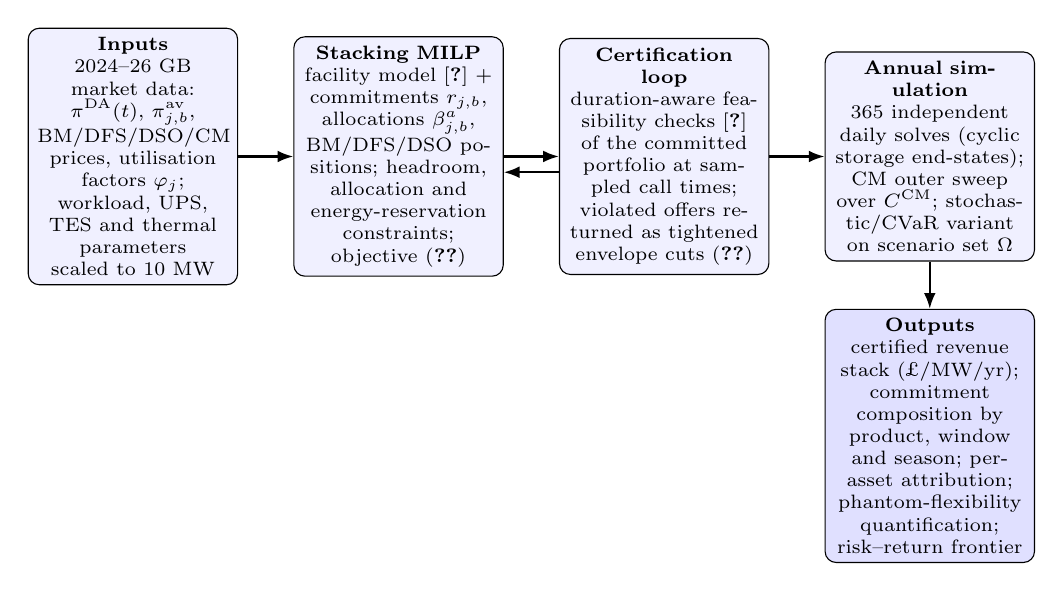
\begin{tikzpicture}[
node distance=6mm and 7mm,
box/.style={draw, rounded corners, align=center, font=\scriptsize, minimum height=10mm, text width=0.20\textwidth, fill=blue!6},
outbox/.style={draw, rounded corners, align=center, font=\scriptsize, minimum height=10mm, text width=0.20\textwidth, fill=blue!12},
arr/.style={-{Latex[length=2mm]}, thick}
]
\node[box] (inputs) {\textbf{Inputs}\\ 2024--26 GB market data: $\pi^{\mathrm{DA}}(t)$, $\pi^{\mathrm{av}}_{j,b}$, BM/DFS/DSO/CM prices, utilisation factors $\varphi_j$; workload, UPS, TES and thermal parameters scaled to 10 MW};
\node[box, right=of inputs] (stack) {\textbf{Stacking MILP}\\ facility model \cite{takci2026characterisation} $+$ commitments $r_{j,b}$, allocations $\beta^a_{j,b}$, BM/DFS/DSO positions; headroom, allocation and energy-reservation constraints; objective \eqref{eq:objective}};
\node[box, right=of stack] (certify) {\textbf{Certification loop}\\ duration-aware feasibility checks \cite{takci2026characterisation} of the committed portfolio at sampled call times; violated offers returned as tightened envelope cuts \eqref{eq:envelope_dn}};
\node[box, right=of certify] (annual) {\textbf{Annual simulation}\\ 365 independent daily solves (cyclic storage end-states); CM outer sweep over $C^{\mathrm{CM}}$; stochastic/CVaR variant on scenario set $\Omega$};
\node[outbox, below=of annual] (out2) {\textbf{Outputs}\\ certified revenue stack (\pounds/MW/yr); commitment composition by product, window and season; per-asset attribution; phantom-flexibility quantification; risk--return frontier};
\draw[arr] (inputs) -- (stack);
\draw[arr] (stack) -- (certify);
\draw[arr] ([yshift=-2mm]certify.west) -- ([yshift=-2mm]stack.east);
\draw[arr] (certify) -- (annual);
\draw[arr] (annual) -- (out2);
\end{tikzpicture}
\caption{Workflow of the revenue-stacking framework. The stacking MILP co-optimises the facility schedule and market commitments; the certification loop verifies duration-deliverability of every commitment against the magnitude--duration envelope of the companion paper and returns cuts until the portfolio is certified; the annual simulation repeats the certified daily problem across two years of GB market data. The daily problem is solved both as a full-information co-optimisation (benchmark B4, the upper bound) and gate-sequentially, with within-day products limited to the residual flexibility left by the day-ahead stage (benchmark B5).}
\label{fig:workflow}
\end{figure*}

\subsection{Facility Model}\label{sec:facility}

The facility model is the integrated MILP developed and validated in \cite{takci2026characterisation}, comprising IT workload scheduling, UPS energy storage and cooling thermodynamics with thermal energy storage, discretised into 15-minute slots over a 24-hour horizon $T$ with a 3-hour extension $T^{\mathrm{ext}} \setminus T$ that accommodates deferred workload and storage recovery. Its constraints are restated here in compact form, both for completeness and because the market layer couples directly to its variables; full derivations, parameter provenance and validation are given in \cite{takci2026characterisation}.

The facility's total grid draw, the quantity every market product acts upon, aggregates the IT, cooling, storage-charging and auxiliary loads:
\begin{flalign}
& P^{\mathrm{Grid}}(t) = P^{\mathrm{Grid}}_{\mathrm{IT}}(t) + P^{\mathrm{Grid}}_{\mathrm{OD}} + P^{\mathrm{UPS}}_{\mathrm{ch}}(t) \notag \\
& \qquad + P^{\mathrm{Chil}\text{-}\mathrm{CRAC}}(t) + P^{\mathrm{Chil}\text{-}\mathrm{TES}}(t), \quad \forall t \in T^{\mathrm{ext}} & \label{eq:grid_power}
\end{flalign}

\subsubsection{IT workload}
Flexible IT jobs originating in slot $t$ are decomposed into tranches $k \in K$ with maximum deferral durations $D_k \in \{0.5, 1, 2, 3\}$~hours, and scheduled through the decision variable $u(t,k,s)$, the CPU utilisation of tranche $k$ executed in slot $s$ within the feasible window $W_{t,k}$. Each job's computational demand must be executed in full within its window, and the total utilisation in any slot may not exceed capacity:
\begin{flalign}
& \sum_{s \in W_{t,k}} u(t,k,s)\,\Delta t = R_t\,\alpha_{t,k}, \quad \forall t \in T,\ \forall k \in K & \label{eq:job_completion} \\
& u^{\mathrm{inflex}}(t) + \sum_{k=1}^{K}\sum_{j=0}^{D_k} u(t\!-\!j,k,s)\big|_{s=t} \leq u_{\max}, \ \ \forall t \in T^{\mathrm{ext}} & \label{eq:cpu_capacity}
\end{flalign}
IT power follows the superlinear utilisation--power relationship, linearised in the implementation by an SOS2 piecewise approximation \cite{takci2026characterisation,dayarathna2015data}:
\begin{flalign}
& P^{\mathrm{IT}}(t) = P^{\mathrm{IT}}_{\mathrm{idle}} + \left(P^{\mathrm{IT}}_{\mathrm{max}} - P^{\mathrm{IT}}_{\mathrm{idle}}\right) u(t)^{1.32} & \label{eq:power_it}
\end{flalign}
where $u(t)$ is the total scheduled utilisation in slot $t$. The IT load is served jointly by the grid and the UPS:
\begin{flalign}
& P^{\mathrm{IT}}(t) = P^{\mathrm{Grid}}_{\mathrm{IT}}(t) + P^{\mathrm{UPS}}_{\mathrm{disch}}(t), \quad \forall t \in T^{\mathrm{ext}} & \label{eq:it_balance}
\end{flalign}

\subsubsection{UPS energy storage}
The UPS battery evolves according to the standard efficiency-adjusted energy balance, with converter limits, mutually exclusive charging and discharging, a resilience floor $E^{\mathrm{UPS}}_{\mathrm{min}} = SoC_{\min} E^{\mathrm{UPS}}_{\mathrm{base}}$ that preserves the backup function at all times, and a cyclic end-state condition:
\begin{flalign}
& E^{\mathrm{UPS}}(t\!+\!\Delta t) = E^{\mathrm{UPS}}(t) + \eta^{\mathrm{UPS}}_{\mathrm{ch}} P^{\mathrm{UPS}}_{\mathrm{ch}}(t)\Delta t - \frac{P^{\mathrm{UPS}}_{\mathrm{disch}}(t)}{\eta^{\mathrm{UPS}}_{\mathrm{disch}}}\Delta t & \label{eq:ups_dyn} \\
& z^{\mathrm{UPS}}_{\mathrm{ch}}(t) P^{\mathrm{UPS}}_{\mathrm{ch,min}} \leq P^{\mathrm{UPS}}_{\mathrm{ch}}(t) \leq z^{\mathrm{UPS}}_{\mathrm{ch}}(t) P^{\mathrm{UPS}}_{\mathrm{ch,max}} & \label{eq:ups_ch_lim} \\
& z^{\mathrm{UPS}}_{\mathrm{disch}}(t) P^{\mathrm{UPS}}_{\mathrm{disch,min}} \leq P^{\mathrm{UPS}}_{\mathrm{disch}}(t) \leq z^{\mathrm{UPS}}_{\mathrm{disch}}(t) P^{\mathrm{UPS}}_{\mathrm{disch,max}} & \label{eq:ups_disch_lim} \\
& z^{\mathrm{UPS}}_{\mathrm{ch}}(t) + z^{\mathrm{UPS}}_{\mathrm{disch}}(t) \leq 1, \qquad E^{\mathrm{UPS}}_{\mathrm{min}} \leq E^{\mathrm{UPS}}(t) \leq E^{\mathrm{UPS}}_{\mathrm{max}} & \label{eq:ups_excl}
\end{flalign}
all $\forall t \in T^{\mathrm{ext}}$.

\subsubsection{Cooling system and thermal storage}
The cooling model couples a chiller, a CRAC unit and a TES tank to the four thermal masses of the facility (IT equipment, racks, cold aisle, hot aisle). Cooling supplied to the CRAC comes directly from the chiller or from TES discharge, both governed by the chiller coefficient of performance, with the chiller electrically capped and the TES following an efficiency-adjusted thermal energy balance:
\begin{flalign}
& Q_{\mathrm{cool}}(t) = P^{\mathrm{Chil}\text{-}\mathrm{CRAC}}(t)\,\mathrm{COP} + Q^{\mathrm{TES}\text{-}\mathrm{CRAC}}(t) & \label{eq:cool_balance} \\
& P^{\mathrm{Chil}\text{-}\mathrm{CRAC}}(t) + P^{\mathrm{Chil}\text{-}\mathrm{TES}}(t) \leq P^{\mathrm{Chiller}}_{\mathrm{max}} & \label{eq:chiller_cap} \\
& E^{\mathrm{TES}}(t) = E^{\mathrm{TES}}(t\!-\!1) + \Big(\eta^{\mathrm{TES}}_{\mathrm{ch}}\,\mathrm{COP}\,P^{\mathrm{Chil}\text{-}\mathrm{TES}}(t\!-\!1) \notag \\
& \qquad\qquad - \frac{Q^{\mathrm{TES}\text{-}\mathrm{CRAC}}(t\!-\!1)}{\eta^{\mathrm{TES}}_{\mathrm{dis}}}\Big)\Delta t & \label{eq:tes_dyn}
\end{flalign}
all $\forall t \in T^{\mathrm{ext}}$. The temperatures of the four thermal nodes evolve according to the discrete-time heat-balance dynamics of \cite{takci2026characterisation,cupelli2018data}, and all temperatures are bounded within their operational ranges, most importantly the cold-aisle band that guarantees IT service quality:
\begin{flalign}
& T_{j'}^{\min} \leq T_{j'}(t) \leq T_{j'}^{\max}, \quad \forall j' \in \{\mathrm{Ain, CA, R, IT, HA}\},\ \forall t & \label{eq:temp_bounds}
\end{flalign}
It is the thermal inertia represented by these bounded states, together with the TES, that permits the cooling load to deviate temporarily from the instantaneous heat load, and it is precisely this buffering that the market layer monetises as duration extension.

\subsection{Market Products and Commitment Variables}\label{sec:products}

Each product $j \in J$ is characterised by its direction (turn-down set $J^{\downarrow}$ or turn-up set $J^{\uparrow}$), its required sustain duration $\tau_j$, its response-speed class, and its procurement granularity, per Table~\ref{tab:products}. Commitments are made at each product's native granularity: the decision variable $r_{j,b} \geq 0$ denotes the capacity committed to product $j$ in procurement window $b \in B_j$, where $B_j$ comprises EFA blocks for the dynamic response services, settlement periods for BR, and the relevant auction windows for QR and SR. Delivered-energy positions are represented by per-slot variables: BM offers $x^{\mathrm{off}}(t)$ and bids $x^{\mathrm{bid}}(t)$, DFS turn-down and turn-up deliveries $x^{\mathrm{dfs},\downarrow}(t)$ and $x^{\mathrm{dfs},\uparrow}(t)$ defined only on published event slots, and DSO deliveries $x^{\mathrm{dso}}(t)$ defined on tendered availability windows. The CM commitment $C^{\mathrm{CM}}$ is a single annual scalar, fixed within each daily problem and optimised in an outer sweep (Section~\ref{sec:cm}). The delivered-energy variables are within-day recourse decisions: in operation they would be taken after the day-ahead commitments are fixed, BM positions before each settlement period's Gate Closure and DFS deliveries when events are called, and they are treated as second-stage variables in the stochastic formulation of Section~\ref{sec:uncertainty} and as strictly subsequent decisions in benchmark B5. The deterministic model co-optimises them with the day-ahead layer under perfect foresight and its value is interpreted accordingly as an upper bound.

Because response speed distinguishes which assets can back which products, each commitment is explicitly allocated across the facility's assets through allocation shares $\beta^{a}_{j,b}$:
\begin{flalign}
& \sum_{a \in A} \beta^{a}_{j,b} = 1, \qquad \beta^{a}_{j,b} = 0 \ \ \forall (a,j) \notin \mathcal{F}, & \label{eq:allocation}
\end{flalign}
where $\mathcal{F}$ is the feasible asset--product set encoding speed compatibility: sub-second products (DC) may be backed only by the UPS inverter; products requiring delivery within one minute (QR) by the UPS and, as a tested assumption, fast IT power capping; and products with delivery at 15 minutes or slower (SR, BM, DFS, DSO, CM) by any asset. The allocation variables serve two purposes: they permit per-asset headroom and energy-reservation constraints that respect each asset's physics, and they make the attribution of portfolio value to assets, one of the paper's research questions, an output of the optimisation rather than a post-hoc estimate.

\subsection{Headroom and Stacking Constraints}\label{sec:headroom}

The stacking core of the formulation requires that, at every slot, the sum of all commitments and delivered positions in each direction fits within the facility's genuinely available capability in that direction. This capability is built up per asset.

\subsubsection{IT headroom}
The deliverable IT turn-down at slot $t$, sustainable for duration $\tau$, is the difference between the scheduled IT power and the power floor that would remain if all workload with at least $\tau$ hours of remaining deferral slack were deferred. Let the utilisation floor be
\begin{flalign}
& u^{\mathrm{flr}}_{\tau}(t) = u^{\mathrm{inflex}}(t) + \!\!\sum_{\substack{(t',k):\, t \in W_{t',k} \\ t' + D_k - t < \tau}}\!\! u(t',k,s)\big|_{s=t}, & \label{eq:floor_util}
\end{flalign}
that is, the inflexible utilisation plus the flexible executions at $t$ whose windows close within the next $\tau$ hours and which therefore cannot be moved out of a $\tau$-hour delivery event. Passing the floor through the same piecewise power map as \eqref{eq:power_it} yields $P^{\mathrm{flr}}_{\tau}(t)$, and the duration-aware IT headroom follows:
\begin{flalign}
& H^{\mathrm{IT},\downarrow}_{\tau}(t) = P^{\mathrm{IT}}(t) - P^{\mathrm{flr}}_{\tau}(t), \quad \forall t,\ \forall \tau \in \mathcal{D}. & \label{eq:head_it}
\end{flalign}
Because the utilisation--power map is convex, evaluating the floor through the shared SOS2 approximation yields a conservative (under-)estimate of the achievable reduction, which is the safe direction for a deliverability guarantee. IT turn-up headroom is limited to the advancement of already-arrived work and is correspondingly small; consistent with the asymmetry established in \cite{takci2026characterisation}, it is set to the utilisation slack $u_{\max} - u(t)$ mapped through \eqref{eq:power_it} and further restricted by the certification layer.

\subsubsection{UPS headroom}
The UPS can reduce net facility demand by curtailing any scheduled charging and discharging up to its converter limit, and increase demand symmetrically:
\begin{flalign}
& H^{\mathrm{UPS},\downarrow}(t) = P^{\mathrm{UPS}}_{\mathrm{disch,max}} - P^{\mathrm{UPS}}_{\mathrm{disch}}(t) + P^{\mathrm{UPS}}_{\mathrm{ch}}(t) & \label{eq:head_ups_dn} \\
& H^{\mathrm{UPS},\uparrow}(t) = P^{\mathrm{UPS}}_{\mathrm{ch,max}} - P^{\mathrm{UPS}}_{\mathrm{ch}}(t) + P^{\mathrm{UPS}}_{\mathrm{disch}}(t) & \label{eq:head_ups_up}
\end{flalign}
The minimum-power thresholds in \eqref{eq:ups_ch_lim}--\eqref{eq:ups_disch_lim} are neglected in the headroom expressions and enforced ex post in certification; at the 10~MW scale they are small relative to committed volumes. The energy dimension of UPS deliverability is handled separately by the reservations of Section~\ref{sec:reservations}.

\subsubsection{Cooling headroom}
Cooling turn-down is achieved by substituting TES discharge for chiller consumption or by drawing down the thermal inertia of the facility; the former is the firm component and defines the headroom credited to commitments:
\begin{flalign}
& H^{\mathrm{CL},\downarrow}(t) \leq P^{\mathrm{Chil}\text{-}\mathrm{TES}}(t) + P^{\mathrm{Chil}\text{-}\mathrm{CRAC}}(t), & \label{eq:head_cool_dn1} \\
& H^{\mathrm{CL},\downarrow}(t) \leq P^{\mathrm{Chil}\text{-}\mathrm{TES}}(t) + \frac{Q^{\mathrm{TES}\text{-}\mathrm{CRAC}}_{\mathrm{max}} - Q^{\mathrm{TES}\text{-}\mathrm{CRAC}}(t)}{\mathrm{COP}}, & \label{eq:head_cool_dn2} \\
& H^{\mathrm{CL},\uparrow}(t) = P^{\mathrm{Chiller}}_{\mathrm{max}} - P^{\mathrm{Chil}\text{-}\mathrm{CRAC}}(t) - P^{\mathrm{Chil}\text{-}\mathrm{TES}}(t). & \label{eq:head_cool_up}
\end{flalign}
Constraint \eqref{eq:head_cool_dn1} caps the reduction at the scheduled cooling draw; \eqref{eq:head_cool_dn2} requires that curtailed chiller cooling can be replaced by additional TES discharge within the tank's rating, so that cold-aisle temperatures remain within \eqref{eq:temp_bounds}. Thermal-inertia contributions beyond TES substitution are not credited in the headroom but are captured by the envelope certification, again the conservative direction.

\subsubsection{Stacking constraints}
With per-asset headrooms defined, the commitments allocated to each asset must fit within that asset's headroom at every slot of the procurement window, and the aggregate of all commitments and delivered positions must fit within the facility total in each direction. For turn-down, the constraints are nested by duration: at each duration level $\tau \in \mathcal{D}$, all products requiring sustain of at least $\tau$ must fit within the $\tau$-sustainable capability,
\begin{flalign}
& \sum_{j \in J^{\downarrow}} \beta^{\mathrm{IT}}_{j,b(t)}\, r_{j,b(t)}\, \mathbb{1}\{\tau_j \geq \tau\} \leq H^{\mathrm{IT},\downarrow}_{\tau}(t), \quad \forall t,\ \forall \tau \in \mathcal{D} & \label{eq:stack_it} \\
& \sum_{j \in J^{\downarrow}} \beta^{a}_{j,b(t)}\, r_{j,b(t)} \leq H^{a,\downarrow}(t), \quad a \in \{\mathrm{UPS}, \mathrm{CL}\},\ \forall t & \label{eq:stack_asset} \\
& \sum_{j \in J^{\downarrow}} r_{j,b(t)}\, \mathbb{1}\{\tau_j \geq \tau\} + x^{\mathrm{off}}(t) + x^{\mathrm{dfs},\downarrow}(t) + x^{\mathrm{dso}}(t) \notag \\
& \quad + \delta^{\mathrm{CM}} C^{\mathrm{CM}}\, \mathbb{1}_{\mathrm{SS}}(t) \notag \\
& \qquad \leq H^{\mathrm{IT},\downarrow}_{\tau}(t) + H^{\mathrm{UPS},\downarrow}(t) + H^{\mathrm{CL},\downarrow}(t), \quad \forall t,\ \forall \tau \in \mathcal{D} & \label{eq:stack_dn}
\end{flalign}
and symmetrically for turn-up, with the facility's firm import capacity providing an additional hard cap that becomes central to the connection-flexibility analysis:
\begin{flalign}
& \sum_{j \in J^{\uparrow}} r_{j,b(t)} + x^{\mathrm{bid}}(t) + x^{\mathrm{dfs},\uparrow}(t) \leq \sum_{a \in A} H^{a,\uparrow}(t), \quad \forall t & \label{eq:stack_up} \\
& P^{\mathrm{Grid}}(t) + \sum_{j \in J^{\uparrow}} r_{j,b(t)} + x^{\mathrm{bid}}(t) + x^{\mathrm{dfs},\uparrow}(t) \leq P^{\mathrm{conn}}, \quad \forall t & \label{eq:conn_cap}
\end{flalign}
Constraint \eqref{eq:stack_dn} embodies the no-double-commitment rule of Section~\ref{sec:market}: because all commitments and deliveries in a direction draw on a single shared headroom, the same megawatt cannot be sold twice, yet the optimiser retains full freedom to split capacity across products, mirroring the EAC's own co-optimisation. Delivered-energy positions ($x$ variables) are included conservatively at every duration level; DFS deliveries are additionally excluded from headroom offered to other services during event periods, implementing the service's primacy rules.

\subsection{Stored-Energy Reservations}\label{sec:reservations}

Power headroom is necessary but not sufficient: a commitment backed by storage must also reserve the energy to sustain delivery for $\tau_j$. For the UPS, committed turn-down requires dischargeable energy above the resilience floor throughout the window, and committed turn-up requires charging room below the ceiling:
\begin{flalign}
& E^{\mathrm{UPS}}(t) \geq E^{\mathrm{UPS}}_{\mathrm{min}} + \sum_{j \in J^{\downarrow}} \beta^{\mathrm{UPS}}_{j,b(t)}\, r_{j,b(t)}\, \frac{\tau_j}{\eta^{\mathrm{UPS}}_{\mathrm{disch}}}, \quad \forall t & \label{eq:res_ups_dn} \\
& E^{\mathrm{UPS}}(t) \leq E^{\mathrm{UPS}}_{\mathrm{max}} - \sum_{j \in J^{\uparrow}} \beta^{\mathrm{UPS}}_{j,b(t)}\, r_{j,b(t)}\, \tau_j\, \eta^{\mathrm{UPS}}_{\mathrm{ch}}, \quad \forall t & \label{eq:res_ups_up}
\end{flalign}
Analogously, cooling-backed turn-down requires the TES to hold the thermal energy to replace curtailed chiller output for the duration:
\begin{flalign}
& E^{\mathrm{TES}}(t) \geq E^{\mathrm{TES}}_{\mathrm{min}} + \mathrm{COP} \sum_{j \in J^{\downarrow}} \beta^{\mathrm{CL}}_{j,b(t)}\, r_{j,b(t)}\, \frac{\tau_j}{\eta^{\mathrm{TES}}_{\mathrm{dis}}}, \quad \forall t & \label{eq:res_tes}
\end{flalign}
Two remarks are in order. First, these reservations interact with the facility's cost optimisation in a way that is invisible to sequential valuation: holding energy for a response commitment forecloses arbitrage cycling of the same energy, so the model prices the opportunity cost of every reservation endogenously. Second, for the continuously exercised Dynamic Regulation service, the expected energy throughput implied by historical frequency distributions is additionally deducted as a scheduled drain on the reserved energy; it is this throughput, rather than the power rating, that is expected to make DR unattractive for a resilience-floored UPS, and the formulation deliberately includes the product so that the optimiser can reject it on economic grounds rather than by assumption.

The IT asset requires no analogous energy reservation, because the job-completion constraint \eqref{eq:job_completion} already guarantees that deferred work, the ``discharge'' of the IT resource, is repaid within its window; its rebound cost is borne in the objective through the energy purchased at post-event prices. This automatic pricing of the rebound is one of the principal advantages of co-optimising commitments with the schedule rather than valuing services independently.

\subsection{Duration Certification}\label{sec:certification}

The headroom and reservation constraints of Sections~\ref{sec:headroom}--\ref{sec:reservations} are linear, slot-wise conditions. They are conservative in the components they credit (TES substitution only, floor-based IT headroom) but they cannot, by themselves, capture every intertemporal interaction that a sustained delivery event engages: cooling states drift during an event, deferred workload accumulates against future CPU capacity, and post-event recovery must itself be feasible. The companion paper's duration-aware assessment \cite{takci2026characterisation} was designed for exactly this question: for a baseline schedule, a start slot $t_0$ and a requested deviation $\Delta P$, it computes the maximum feasible duration $\tau^{*}(t_0, \Delta P)$ of provision, including a mandatory recovery window, by embedding the deviation as a constraint on the grid-power trajectory and testing feasibility of the full facility model. Inverting the envelope gives the maximum deviation sustainable for a given duration, $\overline{\Delta P}^{\downarrow}(t,\tau)$ and $\overline{\Delta P}^{\uparrow}(t,\tau)$, and deliverability of the stacked portfolio requires the nested conditions
\begin{flalign}
& \sum_{j \in J^{\downarrow}} r_{j,b(t)}\, \mathbb{1}\{\tau_j \geq \tau\} \leq \overline{\Delta P}^{\downarrow}(t,\tau), \quad \forall t,\ \forall \tau \in \mathcal{D} & \label{eq:envelope_dn} \\
& \sum_{j \in J^{\uparrow}} r_{j,b(t)}\, \mathbb{1}\{\tau_j \geq \tau\} \leq \overline{\Delta P}^{\uparrow}(t,\tau), \quad \forall t,\ \forall \tau \in \mathcal{D} & \label{eq:envelope_up}
\end{flalign}
The complication is that the envelope depends on the baseline schedule, which the stacking optimisation itself alters. The formulation therefore employs an iterative certification loop:
\begin{enumerate}
    \item \emph{Solve} the stacking MILP with the linear headroom and reservation constraints \eqref{eq:stack_it}--\eqref{eq:res_tes}, and any accumulated envelope cuts \eqref{eq:envelope_dn}--\eqref{eq:envelope_up}, obtaining a candidate schedule and commitment portfolio.
    \item \emph{Certify} the portfolio: for each committed product and a sample of call times within each committed window, embed a delivery event of magnitude equal to the total simultaneous commitment and duration $\tau_j$ into the facility model, following the Scenario~3 procedure of \cite{takci2026characterisation} with its 12-slot recovery window, and test feasibility.
    \item \emph{Cut and repeat}: for every infeasible case, tighten the corresponding envelope value $\overline{\Delta P}(t,\tau)$ to the largest feasible deviation found by binary search, add the updated constraint, and re-solve. Terminate when all sampled calls are feasible.
\end{enumerate}
The loop converges because each cut strictly reduces the feasible commitment set, which is bounded below by zero, and in practice, because the linear headrooms are already conservative, few iterations are required; the number of iterations and the certification gap, the revenue difference between the first and final portfolios, are reported as results. The gap between the \emph{uncertified} portfolio (step 1 only, with \eqref{eq:envelope_dn}--\eqref{eq:envelope_up} omitted) and the certified portfolio measures the phantom flexibility that a naive stacking model would sell; the associated count of failed delivery simulations is reported alongside it. This certification-versus-optimisation architecture parallels the feasibility concern raised for single-service regulation bidding in \cite{fan2026harnessing}, generalised here to a heterogeneous multi-product portfolio, and connects to the broader flexibility-envelope literature \cite{nosair2015flexibility,riaz2022modelling}.

\subsection{Objective Function}\label{sec:objective}

The daily objective minimises net operating cost: energy and network costs less market revenues. Prices are quoted per MWh and powers in kW, hence the factor $10^{-3}$; window lengths $L_b$ convert availability prices to window revenue.
\begin{figure*}[!t]
\normalsize
\begin{flalign}
\min \quad
& \underbrace{\sum_{t \in T^{\mathrm{ext}}} \frac{\Delta t}{10^{3}}\, \big(\pi^{\mathrm{DA}}(t) + \pi^{\mathrm{N}}(t)\big)\, P^{\mathrm{Grid}}(t)}_{\text{energy purchase and network charges}}
\ - \underbrace{\sum_{j \in J} \sum_{b \in B_j} \frac{\pi^{\mathrm{av}}_{j,b}\, r_{j,b}\, L_b}{10^{3}}}_{\text{availability revenue}}
\ - \underbrace{\sum_{j \in J} \varphi_j\, \frac{\pi^{\mathrm{ut}}_{j}}{10^{3}} \sum_{b \in B_j} r_{j,b}\, L_b}_{\text{expected utilisation revenue}} \notag \\
& - \underbrace{\sum_{t \in T^{\mathrm{ext}}} \frac{\Delta t\, \kappa}{10^{3}} \big(\pi^{\mathrm{off}}(t)\, x^{\mathrm{off}}(t) - \pi^{\mathrm{bid}}(t)\, x^{\mathrm{bid}}(t)\big)}_{\text{Balancing Mechanism (acceptance-weighted)}}
\ - \underbrace{\sum_{t \in \mathcal{E}^{\mathrm{DFS}}} \frac{\Delta t}{10^{3}} \big(\pi^{\mathrm{DFS},\downarrow} x^{\mathrm{dfs},\downarrow}(t) + \pi^{\mathrm{DFS},\uparrow} x^{\mathrm{dfs},\uparrow}(t)\big)}_{\text{Demand Flexibility Service}} \notag \\
& - \underbrace{\sum_{t \in \mathcal{W}^{\mathrm{DSO}}} \frac{\Delta t}{10^{3}}\, \pi^{\mathrm{DSO}}\, x^{\mathrm{dso}}(t)}_{\text{DSO services}}
\ - \underbrace{\frac{\pi^{\mathrm{CM}}\, \delta^{\mathrm{CM}}\, C^{\mathrm{CM}}}{365}}_{\text{Capacity Market (daily share)}} & \label{eq:objective}
\end{flalign}
\hrulefill
\vspace*{4pt}
\end{figure*}
Several modelling choices embedded in \eqref{eq:objective} warrant justification. Availability prices $\pi^{\mathrm{av}}_{j,b}$ are exogenous historical clearing prices; at 10~MW the facility is a price-taker in every included market, an assumption revisited for the 100~MW sensitivity. Expected utilisation revenue is captured through calibrated factors $\varphi_j$, the expected fraction of committed capacity-hours actually called, derived from historical frequency distributions for the dynamic services and from published activation statistics for the reserves; scenario-explicit utilisation replaces this term in the stochastic variant. BM participation is represented as price-taking arbitrage against historical accepted prices, discounted by an acceptance factor $\kappa$ calibrated to the dispatch rates of comparable units; a full dispatch simulation of NESO's balancing decisions is beyond scope and left as an extension. Delivered service energy alters the facility's metered consumption, and settlement of these deviations is assumed to occur at the relevant service's utilisation price, with the facility otherwise balanced. Under this balanced-facility assumption the model carries no separate day-ahead position variable and no imbalance settlement: the metered grid profile \emph{is} the day-ahead purchase, and deviations from it are represented only through the service settlements themselves. A full position/imbalance treatment, which would additionally be required to simulate intraday re-trading of the energy position, is left as an extension, consistent with the exclusion of continuous intraday markets from the product set. Finally, network charges enter only through the residual time-varying distribution component $\pi^{\mathrm{N}}(t)$; no Triad or transmission-residual avoidance revenue exists under the post-2023 charging regime \cite{ofgem2019tcr}, and the model deliberately claims none.

\subsection{Capacity Market Layer}\label{sec:cm}

The CM commitment cycle is annual and cannot be co-optimised within a daily problem. It is instead treated as an outer decision: for each candidate $C^{\mathrm{CM}}$, the annual simulation is run with the standing deliverability requirement embedded through \eqref{eq:stack_dn} and the certified envelope,
\begin{flalign}
& \delta^{\mathrm{CM}}\, C^{\mathrm{CM}} \leq \overline{\Delta P}^{\downarrow}(t, \tau_{\mathrm{SS}}), \quad \forall t \in T, & \label{eq:cm_standing}
\end{flalign}
where $\tau_{\mathrm{SS}}$ is the assumed stress-event duration, and the annual net value is evaluated as CM revenue less the shadow cost that the standing obligation imposes on all other products. Because $C^{\mathrm{CM}}$ is a scalar, a coarse sweep suffices to locate the optimum, and the resulting value curve is itself an informative output: it quantifies how much always-available capacity the facility can certify, which is precisely the quantity a connection agreement with a flexible-operation condition would need to specify.

\subsection{Uncertainty and Risk}\label{sec:uncertainty}

The deterministic formulation values the portfolio under perfect foresight of prices and calls, an upper bound that is standard in the stacking literature but optimistic for operational bidding. Uncertainty is incorporated through a two-stage stochastic extension. First-stage decisions, fixed before the trading day, comprise all capacity commitments $r_{j,b}$ and the day-ahead purchase profile; second-stage decisions, taken per scenario $\omega \in \Omega$, comprise the physical dispatch, including the per-asset backing allocations $\beta^{a}_{j,b}$, which the facility may rearrange internally provided every commitment remains covered, the BM positions and the service deliveries under realised prices, DFS events and utilisation calls. In the implementation the first-stage purchase profile is fixed by pinning the metered grid trajectory to its first-stage value, consistent with the balanced-facility assumption of Section~\ref{sec:objective}. Denoting by $C_\omega$ the net cost \eqref{eq:objective} evaluated in scenario $\omega$, the risk-adjusted objective is
\begin{flalign}
& \min \ \sum_{\omega \in \Omega} p_\omega C_\omega + \lambda \Big( \zeta + \frac{1}{1-q} \sum_{\omega \in \Omega} p_\omega \varsigma_\omega \Big) & \label{eq:stoch_obj} \\
& \varsigma_\omega \geq C_\omega - \zeta, \qquad \varsigma_\omega \geq 0, \quad \forall \omega \in \Omega, & \label{eq:cvar_aux}
\end{flalign}
the standard linearisation of conditional value-at-risk at confidence level $q$ \cite{rockafellar2000optimization}. Sweeping the risk-aversion weight $\lambda$ traces the facility's risk--return frontier, and the deterministic model is recovered as the special case $\lambda = 0$, $|\Omega| = 1$. Scenarios are constructed by joint bootstrap of historical days, preserving the empirical correlation between wholesale prices, response clearing prices and frequency events, and reduced by clustering to a computationally tractable set. Comparing the stochastic solution against the deterministic solution evaluated out of sample quantifies the foresight premium embedded in perfect-information valuations, which is reported as a headline result.

\subsection{Evaluation Framework}\label{sec:evaluation}

To isolate the value of the framework's two distinguishing features, co-optimisation and certification, the certified portfolio is benchmarked against a ladder of restricted strategies, each evaluated on identical data:
\begin{enumerate}
    \item[B0.] \emph{Energy-only}: the cost-minimising schedule of \cite{takci2026characterisation} with no service participation, the direct continuation of the companion paper and the natural baseline;
    \item[B1.] \emph{Dedicated assets}: each asset committed wholly to its single best product (UPS to DC, IT to energy arbitrage), representing current industry practice where participation exists;
    \item[B2.] \emph{Greedy sequential stacking}: products committed in descending order of standalone value, each taking the residual capability, representing valuation-by-spreadsheet;
    \item[B3.] \emph{Uncertified co-optimisation}: the full model without the certification loop, whose excess commitments quantify phantom flexibility;
    \item[B4.] \emph{Certified co-optimisation}: the full framework solved as a single full-information problem, giving the value-maximal deliverable portfolio and the upper bound of the ladder;
    \item[B5.] \emph{Market-sequential certified strategy}: decisions taken strictly in gate order. The day-ahead stage co-optimises the energy profile and all availability commitments with the within-day products unavailable; the resulting certified commitments and schedule are then fixed, and BM and DFS positions are optimised over the residual deliverable headroom only. B5 represents implementable sequential operation, and the B4--B5 gap prices the foresight of within-day opportunities that the full-information co-optimisation assumes.
\end{enumerate}
Portfolio value is decomposed by product and by asset using the allocation variables, and the marginal value of each asset is computed by leave-one-out re-optimisation; the difference between the sum of standalone asset values and the portfolio value measures the cross-asset synergies, the monetised counterpart of the physical interactions identified in \cite{takci2026characterisation}.

\subsection{Implementation and Tractability}\label{sec:implementation}

The model is implemented in Python using the Pyomo modelling library and solved with the SCIP solver, retaining the implementation stack of \cite{takci2026characterisation}. The market layer adds, per day, of the order of $10^2$ commitment and allocation variables and $10^3$ linear constraints to the facility model's roughly $3.5 \times 10^3$ continuous variables, $2 \times 10^2$ binaries and SOS2 sets, and the daily problem solves in seconds. Annual runs comprise 365 independent daily solves with storage states rolled between days, parallelised across processes; the certification loop multiplies the daily effort by the number of sampled call checks, each a small fixed-baseline feasibility problem of the Scenario~3 form. The stochastic variant scales the physical block by $|\Omega| \leq 20$; where the UPS minimum-power binaries are not binding, they are relaxed to continuous variables after validation on sample days. Solve statistics are reported alongside the results.

% ======================================================================
\section{Case Study and Data}\label{sec:casestudy}
% ======================================================================

\textit{[To be completed after the modelling stage. This section will specify: (i) the 10~MW facility, scaled from the companion paper's 1~MW case by rack replication with recomputed lumped thermal parameters, a 12~MW firm connection, a 6~MWh/2.7~MW-charge/27~MW-discharge UPS with a 50\% resilience floor, and a 10~MWh$_{\mathrm{th}}$ TES; (ii) the 2024--2026 GB market dataset (day-ahead prices, EAC auction results, BR/QR/SR clearing prices, BM accepted prices and dispatch rates, DFS events, CM parameters, DSO tenders, 1~s frequency data) with sources and retrieval dates; (iii) calibration of $\varphi_j$ and $\kappa$; and (iv) the scenario and sensitivity design, including frequency-response price regimes, flexible-workload share, UPS resilience floor, facility scale (10 vs.\ 100~MW), DSO-zone siting, and connection capacity.]}

% ======================================================================
\section{Results and Discussion}\label{sec:results}
% ======================================================================

\textit{[To be completed after the modelling stage. Planned structure: representative-day mechanics; annual certified revenue stack and composition; per-asset attribution and synergies; value-of-co-optimisation ladder (B0--B5) including phantom flexibility and the sequential-operation gap; risk--return frontier and foresight premium; sensitivity tornado; connection-capacity trade-off; benchmarking of the UPS slice against GB battery revenue indices \cite{modo2026benchmark}.]}

% ======================================================================
\section{Conclusion}\label{sec:conclusion}
% ======================================================================

\textit{[To be completed after the results stage.]}

% ======================================================================
\section*{Suggested Figures (working section --- remove before submission)}
% ======================================================================

The following figures are proposed to support the sections drafted above. Fig.~\ref{fig:workflow} (already included as native Ti\emph{k}Z) covers the overall architecture.

\begin{enumerate}
    \item \textbf{Speed--duration product map (Section~\ref{sec:market}).} A two-dimensional chart with response time on a logarithmic x-axis (100~ms to hours) and required sustain duration on the y-axis, plotting every product in Table~\ref{tab:products} as a labelled box, and overlaying shaded capability regions for each facility asset (UPS: fast/short; IT: slow/long; TES: intermediate). This single figure would communicate the paper's central layering insight, that the optimal stack is a portfolio sorted by response speed, before any mathematics.
    \item \textbf{Facility-and-markets schematic (Sections~\ref{sec:market}--\ref{sec:methodology}).} An extension of the companion paper's data centre layout figure, adding the market interfaces: arrows from each asset to the products it can back, annotated with the allocation variables $\beta^{a}_{j,b}$, and the grid connection cap $P^{\mathrm{conn}}$.
    \item \textbf{Envelope-with-product-boxes overlay (Section~\ref{sec:certification}).} The magnitude--duration envelope $\tau^{*}(t_0, \Delta P)$ heatmap from the companion paper for a representative day, overlaid with rectangles representing each product's $(\tau_j, r_{j,b})$ requirement at its committed level. Products inside the envelope are certified; any protruding rectangle visualises phantom flexibility. This is the visual bridge between the two papers.
    \item \textbf{Committed-capacity Gantt chart (Section~\ref{sec:headroom}).} For a representative day: stacked horizontal bars per EFA block / settlement period showing how the facility's headroom is allocated across DC, DM, BR, QR, SR, BM and energy arbitrage, with the baseline grid-power profile beneath. Demonstrates the no-double-commitment constraint in action.
    \item \textbf{Headroom decomposition time series (Section~\ref{sec:headroom}).} $H^{a,\downarrow}(t)$ and $H^{a,\uparrow}(t)$ for the three assets over 24~h under the cost-optimal schedule, showing when each asset's capability is available and how the committed portfolio consumes it.
    \item \textbf{Annual revenue waterfall (Section~\ref{sec:results}).} From the energy-only cost baseline (B0), successive bars adding arbitrage reshaping, response, reserve, BM, DFS, DSO and CM revenues to the certified total, in \pounds/MW/yr; the headline ``money chart''.
    \item \textbf{Stack composition heatmap (Section~\ref{sec:results}).} Committed MW by product (rows) against EFA block and season (columns), revealing the temporal structure of the optimal stack.
    \item \textbf{Value-of-co-optimisation ladder (Section~\ref{sec:evaluation}).} Bar chart of B0--B5 annual values, with B3 annotated by the phantom-flexibility volume (MWh of undeliverable commitments) that certification removes, and the B4--B5 gap annotated as the value of within-day foresight.
    \item \textbf{Per-asset attribution and synergy matrix (Section~\ref{sec:evaluation}).} Left panel: leave-one-out marginal value of each asset; right panel: a $3\times3$ matrix of pairwise synergies (portfolio value minus sum of parts).
    \item \textbf{Risk--return frontier (Section~\ref{sec:uncertainty}).} Expected annual net value against CVaR$_{0.95}$ as $\lambda$ is swept, with the deterministic perfect-foresight point marked to visualise the foresight premium.
    \item \textbf{Connection-capacity trade-off curve (Sections~\ref{sec:cm} and \ref{sec:results}).} Annual portfolio value against firm import capacity $P^{\mathrm{conn}}$ swept below the nominal 12~MW, quantifying the revenue cost of accepting a smaller or non-firm connection; the policy figure for the flexible-connections agenda.
    \item \textbf{Certification-loop convergence (Section~\ref{sec:certification}).} Portfolio revenue and number of infeasible delivery checks per iteration of the certification loop, evidencing convergence and the size of the certification gap.
\end{enumerate}

% -------- Bibliography --------
\bibliographystyle{IEEEtran}
\bibliography{references}

% --- Acknowledgements Section ---
\section*{Acknowledgements}

This work was supported by the Engineering and Physical Sciences Research Council (EPSRC) and the Economic and Social Research Council (ESRC) through funding provided to the Energy Demand Research Centre (grant number EP/Y010078/1).

\end{document}
